\chapter{Experimentación} 

Con el fin de dar evidencia a favor de la hipótesis, se diseñaron dos experimentos siguiendo la metodología del diseño multifactorial\cite{Montgomery2001}.
%En estos, la idea es medir la sensibilidad de las respuestas: tiempo de extracción y precisión de la clasificación cuando los parámetros de frecuencia se alejan de la configuración original de $\Delta \tau$=1, $\Delta \rho$=1 $\Delta \phi$=1º.

Los resultados de ambos experimentos se estudiaran por medio de un \textbf{Análisis de Varianza}\cite{Montgomery2001} (ANOVA por sus siglas en inglés). Aquí se toman $n$ muestras de $k$ poblaciones y estos datos se estudian para confirmar que vienen de un mismo origen (o sea, que todos se comportan estadísticamente igual) o no.

Es necesario establecer una hipótesis nula y una alternativa:
\begin{itemize}
    \item Hipótesis nula $H_0$: la media entre los grupos estudiados es la misma y no afecta el resultado.
    
    $\mu_0 = \mu_1 = ... = \mu_n$.
    \item Hipótesis alternativa $H_1$: la media de al menos uno de los grupos estudiados es diferente y afecta el resultado.
    
    $\exists i,j / \mu_i \neq \mu_j$.
\end{itemize}


\section{Experimento A: Tiempo de ejecución de la extracción de características}

El primer experimento se realizó para medir la influencia de los parámetros de frecuencia y del tipo de cobertura de terreno sobre la variable de respuesta, el \textbf{tiempo requerido para generar las características} de una imagen. Siguiendo el modelo multifactorial\cite{Montgomery2001}, los niveles y factores para el experimento A fueron:
\begin{itemize}
    \item $\Delta \tau$ (píxeles): 1, 2 y 3.
    \item $\Delta \rho$ (píxeles): 1, 2 y 3.
    \item $\Delta \phi$ (grados): 0,5º, 1º y 2º.
    \item Cobertura de terreno (tipos): bosque, agua, rural, urbano y sembradío.
\end{itemize}

Con 32 imágenes por tipo de cobertura y los niveles de las variables anteriores, se tienen 4320 ($3\times3\times3\times32\times5$) ejecuciones por cada una de las tres réplicas. Esto suma un gran total de 12960 ejecuciones de la TT.

Por cada ejecución de la TT se producen dos resultados: un arreglo de TF por cada imagen y el tiempo de ejecución de la extracción de características. El primero se utilizó para el experimento B y el segundo se evaluó con ANOVA.

A continuación se explican los detalles del experimento A.

\subsection{Conjunto de imágenes}

Las imágenes utilizadas para la extracción de características provienen del proyecto Carta 2005\cite{CARTA} y fueron proporcionadas por el PRIAS. A su vez, éstas fueron recortadas y clasificadas previamente por un experto geógrafo. 

Se contó con 32 imágenes por tipo de cobertura, lo que suma 160 imágenes en total. Cada imagen tiene una dimensión de $500 \times 500$ píxeles almacenadas en formato PNG y se eligió este tamaño previendo el tiempo de extracción de alrededor 130 segundos por imagen, según \cite{Garita2013}.

El cuadro \ref{fig:types} muestra diferentes ejemplos de cada tipo de textura. En la primera fila se muestran texturas más homogéneas y en la segunda filas texturas más heterogéneas de cada tipo de cobertura.

%\begin{figure}[h]
%    \centering
    \begin{table}
    \setlength{\tabcolsep}{0.2pt}
    \renewcommand{\arraystretch}{0.1}
        \begin{tabular}{ ccccc }
            
            
            
\includegraphics[width=0.2\textwidth]{images/tipos/Au.png}& 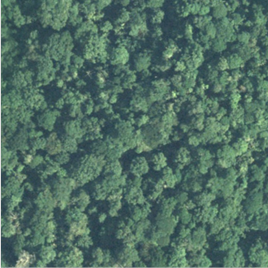
\includegraphics[width=0.2\textwidth]{images/tipos/Bu.png}& 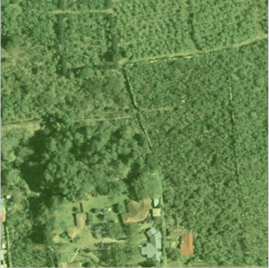
\includegraphics[width=0.2\textwidth]{images/tipos/Ru.png}& 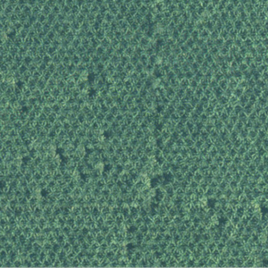
\includegraphics[width=0.2\textwidth]{images/tipos/Pu.png}& 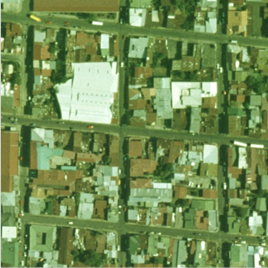
\includegraphics[width=0.2\textwidth]{images/tipos/Uu.png}\\
            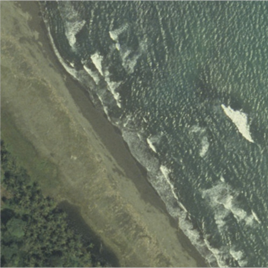
\includegraphics[width=0.2\textwidth]{images/tipos/Ad.png}& 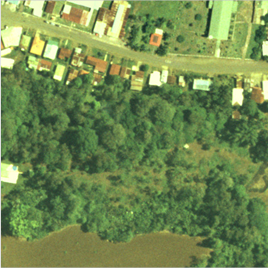
\includegraphics[width=0.2\textwidth]{images/tipos/Bd.png}& 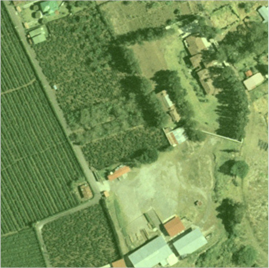
\includegraphics[width=0.2\textwidth]{images/tipos/Rd.png}& 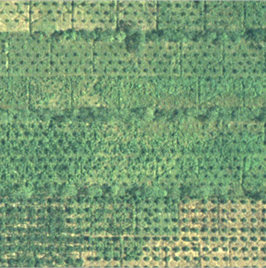
\includegraphics[width=0.2\textwidth]{images/tipos/Pd.png}& 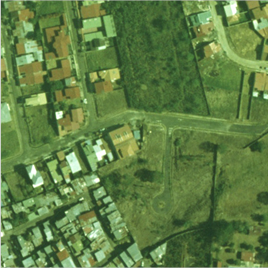
\includegraphics[width=0.2\textwidth]{images/tipos/Ud.png}\\
            &&&&\\
            &&&&\\
            &&&&\\
            Agua & Bosque & Rural & Sembradío & Urbano \\
            
        \end{tabular}
        \caption{Ejemplo de tipos de cobertura. Cada columna presenta dos imágenes de un tipo de cobertura distinto, respectivamente: agua, bosque, rural, sembradío y urbano.}
        \label{fig:types}
    \end{table}
    
    %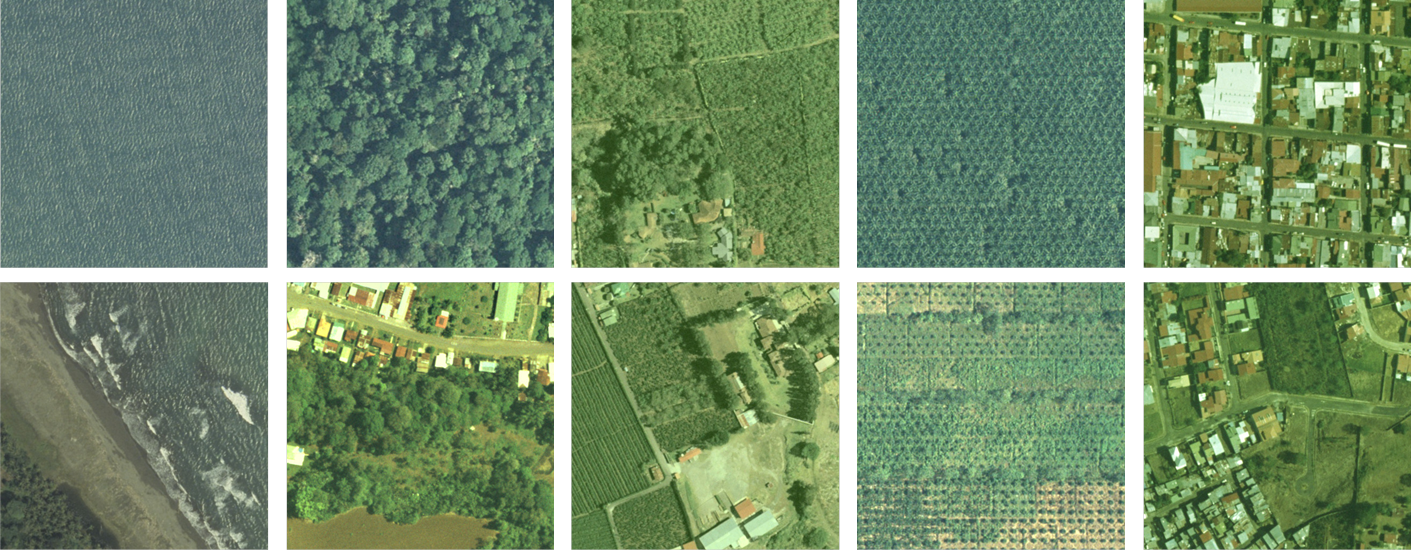
\includegraphics[width=1\textwidth]{images/tipos.png}
    
%\end{figure}


\subsection{Funcionales}

Las funcionales utilizadas en cada uno de los tres pasos de reducción son críticas para extraer características útiles para la etapa de clasificación y puede en realidad ser un tema de investigación por sí solo. Es por esto que las funcionales que se utilizaron en el experimento A son aquellas que mostraron buenos resultados al clasificar texturas en \cite{Petrou2007} y \cite{Tutorial2008}.\\

\begin{longtable}{ |c|l| }
        \hline 
        \textbf{\#} & \textbf{Funcional} \\
        \hline 
        \endhead
        
    	1.&$\sum \limits_{i=1}^{N}{x_i}$ \\ \hline
    	2.&$\sum \limits_{i=1}^{N}{ix_i}$\\ \hline
    	3.&$\frac{1}{N}\sqrt{\sum \limits_{i=1}^{N}{(x_i-\hat{x})^2}}$  \\ \hline
    	4.&$\sqrt{\sum \limits_{i=1}^{N}{x_i^2}}$  \\ \hline
    	5.&$\max \limits_{ i=1}^{N}{x_i}$  \\ \hline
    	6.&$\sum \limits_{i=1}^{N-1}{|{x_{i+1}-x_i}|}$  \\ \hline
    	7.&$\sum \limits_{i=1}^{N-1}{|{x_{i+1}-x_i}|}^2$  \\ \hline
    	8.&$\sum \limits_{i=4}^{N-3}{|{x_{i-3}+x_{i-2}+x_{i-1}-x_{i+1}-x_{i+2}-x_{i+3}}|}$  \\ \hline
    	9.&$\sum \limits_{i=3}^{N-2}{|{x_{i-2}+x_{i-1}-x_{i+1}-x_{i+2}}|}$  \\ \hline
    	10.&$\sum \limits_{i=5}^{N-4}{|{x_{i-4}+x_{i-3}+...+x_{i-1}-x_{i+1}-...-x_{i+3}-x_{i+4}}|}$  \\ \hline
    	11.&$\sum \limits_{i=6}^{N-5}{|{x_{i-5}+x_{i-4}+...+x_{i-1}-x_{i+1}-...-x_{i+4}-x_{i+5}}|}$  \\ \hline
    	12.&$\sum \limits_{i=7}^{N-6}{|{x_{i-6}+x_{i-5}+...+x_{i-1}-x_{i+1}-...-x_{i+5}-x_{i+6}}|}$  \\ \hline
    	13.&$\sum \limits_{i=8}^{N-7}{|{x_{i-7}+x_{i-6}+...+x_{i-1}-x_{i+1}-...-x_{i+6}-x_{i+7}}|}$  \\ \hline
    	14.&$\sum \limits_{i=5}^{N-4}\sum \limits_{k=1}^{4}{|{x_{i-k}-x_{i+k}}|}$  \\ \hline
    	15.&$\sum \limits_{i=6}^{N-5}\sum \limits_{k=1}^{5}{|{x_{i-k}-x_{i+k}}|}$  \\ \hline
    	16.&$\sum \limits_{i=7}^{N-6}\sum \limits_{k=1}^{6}{|{x_{i-k}-x_{i+k}}|}$  \\ \hline
    	17.&$\sum \limits_{i=8}^{N-7}\sum \limits_{k=1}^{7}{|{x_{i-k}-x_{i+k}}|}$  \\ \hline
    	18.&$\sum \limits_{i=11}^{N-10}\sum \limits_{k=1}^{10}{|{x_{i-k}-x_{i+k}}|}$  \\ \hline
    	19.&$\sum \limits_{i=16}^{N-15}\sum \limits_{k=1}^{15}{|{x_{i-k}-x_{i+k}}|}$  \\ \hline
    	20.&$\sum \limits_{i=21}^{N-20}\sum \limits_{k=1}^{20}{|{x_{i-k}-x_{i+k}}|}$  \\ \hline
    	21.&$\sum \limits_{i=26}^{N-25}\sum \limits_{k=1}^{25}{|{x_{i-k}-x_{i+k}}|}$  \\ \hline
    	22.&$\sum \limits_{i=11}^{N-10}((1+\sum \limits_{k=1}^{10}{|{x_{i-k}-x_{i+k}})/(1+\sum \limits_{k=-10}^{9}{|{x_{i-k}-x_{i+k}}|}}))$  \\ \hline
    	23.&$\sum \limits \limits_{i=11}^{N-10}\sqrt{|(\sum \limits_{k=1}^{10}{|{x_{i-k}-x_{i+k}})^2/(1+\sum \limits_{k=-10}^{9}{|{x_{i-k}-x_{i+k}}|}})|}$  \\ \hline
    	24.&$\sum \limits_{i=1}^{N-2}{|{x_{i}-2x_{i+1}+x_{i+2}}|}$  \\ \hline
    	25.&$\sum \limits_{i=1}^{N-3}{|{x_{i}-3x_{i+1}+3x_{i+2}-x_{i+3}}|}$  \\ \hline
    	26.&$\sum \limits_{i=1}^{N-4}{|{x_{i}-4x_{i+1}+6x_{i+2}-4x_{i+3}+x_{i+4}}|}$  \\ \hline
    	27.&$\sum \limits_{i=1}^{N-5}{|{x_{i}-5x_{i+1}+10x_{i+2}-10x_{i+3}+5x_{i+4}-x_{i+4}}|}$  \\ \hline
    	28.&$\sum \limits_{i=1}^{N-2}{|{x_{i}-2x_{i+1}+x_{i+2}}x_{i+1}|}$  \\ \hline
    	29.&$\sum \limits_{i=1}^{N-3}{|{x_{i}-3x_{i+1}+3x_{i+2}-x_{i+3}}x_{i+1}|}$  \\ \hline
    	30.&$\sum \limits_{i=1}^{N-4}{|{x_{i}-4x_{i+1}+6x_{i+2}-4x_{i+3}+x_{i+4}}x_{i+2}|}$  \\ \hline
    	31.&$\sum \limits_{i=1}^{N-5}{|{x_{i}-5x_{i+1}+10x_{i+2}-10x_{i+3}+5x_{i+4}-x_{i+4}}x_{i+2}|}$ \\ \hline
    \caption{Funcionales de trazo utilizadas en la extracción de características.}
    \label{tab:ft}
\end{longtable}


%Las 31 funcionales de trazo utilizadas fueron:
%\begin{enumerate}
%\item $\sum \limits_{i=1}^{N}{x_i}$ 
%\item $\sum \limits_{i=1}^{N}{ix_i}$
%\item $\frac{1}{N}\sqrt{\sum \limits_{i=1}^{N}{(x_i-\hat{x})^2}}$  
%\item $\sqrt{\sum \limits_{i=1}^{N}{x_i^2}}$  
%\item $\max \limits_{ i=1}^{N}{x_i}$  
%\item $\sum \limits_{i=1}^{N-1}{|{x_{i+1}-x_i}|}$  
%\item $\sum \limits_{i=1}^{N-1}{|{x_{i+1}-x_i}|}^2$  
%\item $\sum \limits_{i=4}^{N-3}{|{x_{i-3}+x_{i-2}+x_{i-1}-x_{i+1}-x_{i+2}-x_{i+3}}|}$  
%\item $\sum \limits_{i=3}^{N-2}{|{x_{i-2}+x_{i-1}-x_{i+1}-x_{i+2}}|}$  
%\item $\sum \limits_{i=5}^{N-4}{|{x_{i-4}+x_{i-3}+...+x_{i-1}-x_{i+1}-...-x_{i+3}-x_{i+4}}|}$  
%\item $\sum \limits_{i=6}^{N-5}{|{x_{i-5}+x_{i-4}+...+x_{i-1}-x_{i+1}-...-x_{i+4}-x_{i+5}}|}$  
%\item $\sum \limits_{i=7}^{N-6}{|{x_{i-6}+x_{i-5}+...+x_{i-1}-x_{i+1}-...-x_{i+5}-x_{i+6}}|}$  
%\item $\sum \limits_{i=8}^{N-7}{|{x_{i-7}+x_{i-6}+...+x_{i-1}-x_{i+1}-...-x_{i+6}-x_{i+7}}|}$  
%\item $\sum \limits_{i=5}^{N-4}\sum \limits_{k=1}^{4}{|{x_{i-k}-x_{i+k}}|}$  
%\item $\sum \limits_{i=6}^{N-5}\sum \limits_{k=1}^{5}{|{x_{i-k}-x_{i+k}}|}$  
%\item $\sum \limits_{i=7}^{N-6}\sum \limits_{k=1}^{6}{|{x_{i-k}-x_{i+k}}|}$  
%\item $\sum \limits_{i=8}^{N-7}\sum \limits_{k=1}^{7}{|{x_{i-k}-x_{i+k}}|}$  
%\item $\sum \limits_{i=11}^{N-10}\sum \limits_{k=1}^{10}{|{x_{i-k}-x_{i+k}}|}$  
%\item $\sum \limits_{i=16}^{N-15}\sum \limits_{k=1}^{15}{|{x_{i-k}-x_{i+k}}|}$  
%\item $\sum \limits_{i=21}^{N-20}\sum \limits_{k=1}^{20}{|{x_{i-k}-x_{i+k}}|}$  
%\item $\sum \limits_{i=26}^{N-25}\sum \limits_{k=1}^{25}{|{x_{i-k}-x_{i+k}}|}$  
%\item $\sum \limits_{i=11}^{N-10}((1+\sum \limits_{k=1}^{10}{|{x_{i-k}-x_{i+k}})/(1+\sum \limits_{k=-10}^{9}{|{x_{i-k}-x_{i+k}}|}}))$  
%\item $\sum \limits \limits_{i=11}^{N-10}\sqrt{|(\sum \limits_{k=1}^{10}{|{x_{i-k}-x_{i+k}})^2/(1+\sum \limits_{k=-10}^{9}{|{x_{i-k}-x_{i+k}}|}})|}$  
%\item $\sum \limits_{i=1}^{N-2}{|{x_{i}-2x_{i+1}+x_{i+2}}|}$  
%\item $\sum \limits_{i=1}^{N-3}{|{x_{i}-3x_{i+1}+3x_{i+2}-x_{i+3}}|}$  
%\item $\sum \limits_{i=1}^{N-4}{|{x_{i}-4x_{i+1}+6x_{i+2}-4x_{i+3}+x_{i+4}}|}$  
%\item $\sum \limits_{i=1}^{N-5}{|{x_{i}-5x_{i+1}+10x_{i+2}-10x_{i+3}+5x_{i+4}-x_{i+4}}|}$  
%\item $\sum \limits_{i=1}^{N-2}{|{x_{i}-2x_{i+1}+x_{i+2}}x_{i+1}|}$  
%\item $\sum \limits_{i=1}^{N-3}{|{x_{i}-3x_{i+1}+3x_{i+2}-x_{i+3}}x_{i+1}|}$  
%\item $\sum \limits_{i=1}^{N-4}{|{x_{i}-4x_{i+1}+6x_{i+2}-4x_{i+3}+x_{i+4}}x_{i+2}|}$  
%\item $\sum \limits_{i=1}^{N-5}{|{x_{i}-5x_{i+1}+10x_{i+2}-10x_{i+3}+5x_{i+4}-x_{i+4}}x_{i+2}|}$ 
%\end{enumerate}


Las 31 funcionales de trazo se presentan en el cuadro \ref{tab:ft}.
Muchas de las funcionales utilizadas aquí exploran un área sobre $\tau$. Por ejemplo, las funcionales 10, 11, 12 y 13 suman, dado el punto de tangencia, el valor de los píxeles en ambas direcciones de la recta; cada vez en un vecindario más grande. Otras funcionales calculan valores interesantes del trazo, el punto máximo (5) o la suma de todos los puntos (1).\\


\begin{longtable}{ |c|l| }
        \hline
        \textbf{\#} & \textbf{Funcional} \\
        \hline
        \endhead
1.&$\max \limits_{i=1}^{N}{x_i}$\\ \hline
2.&$\min \limits_{i=1}^{N}{x_i}$\\ \hline
3.&$\sqrt{\sum \limits_{i=1}^{N}{x_i^2}}$ \\ \hline
4.&$\frac{\sum \limits_{i=1}^{N}{ix_i}}{\sum \limits_{i=1}^{N}{x_i}}$ \\ \hline
5.&$\sum \limits_{i=1}^{N}{ix_i}$ \\ \hline
6.&$\frac{1}{N}\sum_{i=1}^{N}{(x_i-\hat{x})^2}$ \\ \hline
7.&$c$ tal que:$\sum \limits_{i=1}^{c}{x_i}=\sum \limits_{i=c}^{N}{x_i}$ \\ \hline
8.&$\sum \limits_{i=1}^{N-1}{|x_{i+1}-x_{i}|}$ \\ \hline
9.&$c$ tal que:$\sum \limits_{i=1}^{c}{|x_{i+1}-x_{i}|}=\sum \limits_{i=c}^{N-1}{|x_{i+1}-x_{i}|}$ \\ \hline
10.&$\sum \limits_{i=1}^{N-4}{|x_{i}-4x_{i+1}+6x_{i+2}-4x_{i+3}+x_{i+4}|}$ \\ \hline
    \caption{Funcionales diamétricas utilizadas en la extracción de características.}
    \label{tab:fd}
\end{longtable}

%\begin{enumerate}
%\item $\max \limits_{i=1}^{N}{x_i}$
%\item $\min \limits_{i=1}^{N}{x_i}$
%\item $\sqrt{\sum \limits_{i=1}^{N}{x_i^2}}$ 
%\item $\frac{\sum \limits_{i=1}^{N}{ix_i}}{\sum \limits_{i=1}^{N}{x_i}}$ 
%\item $\sum \limits_{i=1}^{N}{ix_i}$ 
%\item $\frac{1}{N}\sum_{i=1}^{N}{(x_i-\hat{x})^2}$ 
%\item $c$ tal que: $\sum \limits_{i=1}^{c}{x_i}=\sum \limits_{i=c}^{N}{x_i}$ 
%\item $\sum \limits_{i=1}^{N-1}{|x_{i+1}-x_{i}|}$ 
%\item $c$ tal que: $\sum \limits_{i=1}^{c}{|x_{i+1}-x_{i}|}=\sum \limits_{i=c}^{N-1}{|x_{i+1}-x_{i}|}$ 
%\item $\sum \limits_{i=1}^{N-4}{|x_{i}-4x_{i+1}+6x_{i+2}-4x_{i+3}+x_{i+4}|}$ 
%\end{enumerate}


Las 10 funcionales de diámetro utilizadas se presentan en el cuadro \ref{tab:fd}.
De estas, algunas son de la misma familia que varias funcionales de trazo, pero aparecen aquí algunas totalmente distintas, como la 7 y la 9. En la 7, se calcula un número $c$ sobre el trazo en donde la suma de los píxeles antes de $c$ sea igual a la suma de los píxeles luego de $c$, esto con el fin de encontrar un punto de equilibrio sobre el trazo. En caso de no existir, se utiliza el valor de 0.\\

%Las 18 funcionales de circo utilizadas fueron:
%\begin{enumerate}
%\item $\sum \limits_{i=1}^{N-1}{|x_{i+1}-x_{i}|^2}$
%\item $\sum \limits_{i=1}^{N-1}{|x_{i+1}-x_{i}|}$
%\item $\sqrt{\sum \limits_{i=1}^{N}{x_i^2}}$ 
%\item $\sum \limits_{i=1}^{N}{x_i}$ 
%\item $\max \limits_{i=1}^{N}{x_i}$ 
%\item $\max \limits_{i=1}^{N}{x_i}-\min \limits_{i=1}^{N}{x_i}$ 
%\item $i$ tal que $x_i=\min \limits_{i=1}^{N}{x_i}$ 
%\item $i$ tal que $x_i=\max \limits_{i=1}^{N}{x_i}$ 
%\item $i$ tal que $x_i=\min \limits_{i=1}^{N}{x_i}$ sin la primera armónica 
%\item $i$ tal que $x_i=\max \limits_{i=1}^{N}{x_i}$ sin la primera armónica 
%\item Amplitud de la primera armónica 
%\item Fase de la primera armónica 
%\item Amplitud de la segunda armónica 
%\item Fase de la segunda armónica 
%\item Amplitud de la tercera armónica 
%\item Fase de la tercera armónica 
%\item Amplitud de la cuarta armónica 
%\item Fase de la cuarta armónica 
%\end{enumerate}


\begin{longtable}{ |c|l| }
        
        \hline
        \textbf{\#} & \textbf{Funcional} \\
        \hline
        \endhead
        
        1.&$\sum \limits_{i=1}^{N-1}{|x_{i+1}-x_{i}|^2}$\\ \hline
    2.&$\sum \limits_{i=1}^{N-1}{|x_{i+1}-x_{i}|}$\\ \hline
    3.&$\sqrt{\sum \limits_{i=1}^{N}{x_i^2}}$ \\ \hline
    4.&$\sum \limits_{i=1}^{N}{x_i}$ \\ \hline
    5.&$\max \limits_{i=1}^{N}{x_i}$ \\ \hline
    6.&$\max \limits_{i=1}^{N}{x_i}-\min \limits_{i=1}^{N}{x_i}$ \\ \hline
    7.&$i$ tal que $x_i=\min \limits_{i=1}^{N}{x_i}$ \\ \hline
    8.&$i$ tal que $x_i=\max \limits_{i=1}^{N}{x_i}$ \\ \hline
    9.&$i$ tal que $x_i=\min \limits_{i=1}^{N}{x_i}$ sin la primera armónica \\ \hline
    10.&$i$ tal que $x_i=\max \limits_{i=1}^{N}{x_i}$ sin la primera armónica \\ \hline
    11.&Amplitud de la primera armónica \\ \hline
    12.&Fase de la primera armónica \\ \hline
    13.&Amplitud de la segunda armónica \\ \hline
    14.&Fase de la segunda armónica \\ \hline
    15.&Amplitud de la tercera armónica \\ \hline
    16.&Fase de la tercera armónica \\ \hline
    17.&Amplitud de la cuarta armónica \\ \hline
    18.&Fase de la cuarta armónica \\ \hline
    
            
    \caption{Funcionales de circo utilizadas en la extracción de características.}
    \label{tab:fc}
\end{longtable}

Las funcionales de circo se presentan en el cuardo \ref{tab:fc} e introducen propiedades de las armónicas de las transformadas diamétricas interpretadas como ondas (de la 11 a la 18). Éstas exponen características físicas que puede facilitar la identificación de las imágenes originales.

\subsection{Implementación del algoritmo de la TT}

La implementación de la TT se basó en el código \cite{Garita2014}. Esta consiste de 3 etapas: 

\begin{enumerate}
    
    \item \textbf{Carga de imágenes}
    %%%%%%%%%%%%%%%%%%%%%%%%%%
    
    Las imágenes se cargan una a la vez, y en el caso de tener que procesar múltiples imágenes se puede utilizar paralelismo a nivel de tareas (programas) y cargar una imagen por cada programa.
    La carga de imágenes se realizó utilizando la biblioteca para manipulación de imágenes \textit{ImageMagick}\footnote{http://www.imagemagick.org/}. Es necesario convertir los píxeles de la imagen a una representación en escala de grises, lo cual se lleva a cabo con la función \texttt{MagickQuantizeImage} \cite{ImageMagick2015}, usando como tercer parámetro \texttt{GRAYColorspace}. Esta función analiza los colores de la imagen y los mapea al espacio lineal de grises usando el algoritmo \texttt{quantize}\cite{quantize2015}. Esto permite utilizar una sola capa de color para el cálculo de las funcionales. Una vez que se haya levantado la imagen en memoria, se pasa a la segunda etapa de preprocesamiento.
    
    
    \item \textbf{Preprocesamiento de las imágenes}
    %%%%%%%%%%%%%%%%%%%%%%%%%%
    
    La etapa de preprocesamiento calcula datos comunes que serán utilizados durante la extracción de características con el fin de no tener que recomputarlos. Aquí es importante tomar en cuenta las características de memoria del equipo donde corre la implementación, ya que por cada imagen se debe almacenar una cantidad considerable de información que tiene una relación directa con el tamaño de la imagen y los parámetros $\Delta$. Estos son:
    \begin{itemize}
        \item Alto y Ancho.
        \item $\Delta \tau$, $\Delta \rho$ y $\Delta \phi$.
        \item Tamaño de la cuadrícula, dependiente de la arquitectura para máximizar el detalle.
        \item Píxel de inicio y fin de cada trazo.
        \item El desplazamiento en los ejes $x$ y $y$ para cada trazo, dependiente de los parámetros $\Delta$.
    \end{itemize}
    
    
    \item  \textbf{Extracción de características}
    %%%%%%%%%%%%%%%%%%%%%%%%%%
    
    Por último, se aplican los tres juegos de funcionales a los datos. Primero, se seleccionan los puntos involucrados en las funcionales de trazo, utilizando los datos precalculados en la etapa anterior, para luego aplicar de forma iterativa todas las funcionales.
    Cada funcional de cada paso (trazo, diamétrica o de circo) podría ser ejecutada de forma independiente ya que la dependencia existe entre cada juego de funcionales y no entre las funcionales de cada juego. El pseudocódigo en el algoritmo \ref{fig:extraccion} muestra este proceso.\\
    
    \begin{algorithm}[h]
    \floatname{algorithm}{Algoritmo}
        \begin{algorithmic}
            \State $I =$ Imagen a procesar
            
            \For{$a$ en ángulos a procesar} 
            
                \For{$d$ en trazos a procesar} 
                    
                    \For{$t$ en puntos a procesar} 
                        \LineComment{Calcular las funcionales de trazo}
                        \State $I_{\tau} = $ calcularFuncionalesTrazo($I$, $a$, $d$, $t$)
                    \EndFor
                \EndFor
    
                \LineComment{Luego de procesadas todas las funcionales de trazo}
                \For{$d$ en trazos a procesar} 
                    \LineComment{Calcular las funcionales diamétricas para cada funcional de trazo}
                    \State $I_{\rho} = $ calcularFuncionalesDiametrica($I_{\tau}$)
                \EndFor
            
            \EndFor
            \LineComment{Luego de procesadas todas las funcionales de trazo y diamétricas}
            
            \For{$a$ en ángulos a procesar} 
                \LineComment{Calcular las funcionales de circo para cada funcional trazo+diamétrica}
                \State $I_{\phi} = $ calcularFuncionalesCirco($I_{\rho}$)
    
            \EndFor
        \end{algorithmic}
        \caption{Procesamiento de la imagen y cálculo de las características triples ($I_{\phi}$)}
        \label{fig:extraccion}
    \end{algorithm}

    La implementación\cite{Garita2014} debió ser modificada, ya que no aceptaba parámetros de frecuencia distintos a los originales. Esto requirió cambiar todos los ciclos cuyo índice o límite tuviera relación con $\Delta \phi = 1$. 

    \begin{figure}
        \begin{lstlisting}
        int phi;
        for (phi = 0; phi < 360; phi++) { ... }
        \end{lstlisting}
        \caption{Ciclo original, utilizando $\Delta \phi =1$.}
        \label{fig:forTT-rgf}
    \end{figure}
    
    
La figura \ref{fig:forTT-rgf} muestra uno de los ciclos originales. En este se puede notar como el bucle toma en cuenta, grado por grado, todas las rotaciones en 360 grados. Luego de modificarse, el limite del ciclo es la variable \textit{\_360EntredPhi}, que se define como la razón de todos los grados en el círculo (360º) y el parámetro de frecuencia $\Delta \phi$, dPhi. En este caso particular, dPhi toma un valor de 3 pero podría ser cualquier otro.
    
    \begin{figure}
        \begin{lstlisting}
        double dPhi = 3; // dPhi puede tomar cualquier valor.
        int phi;
        int _360EntredPhi = 360 / dPhi;
        for (phi = 0; phi < _360EntredPhi; phi++) { ... }
        \end{lstlisting}
        \label{fig:forTT-rrb}
        \caption{Ciclo modificado, utilizando $\Delta \phi = 3$.}
    \end{figure}
    
    Dado que el programa de \cite{Garita2014} se enfocaba en la paralelización, los parámetros de ejecución son dos: la imagen a procesar y la cantidad de hilos o procesos a utilizar para la paralelización. La salida del programa, los TF de cada imagen, eran desplegadas en pantalla.
    Las modificaciones hechas aquí también cambiaron estos comportamientos. Los parámetros necesarios ahora son seis, de los cuales, el segundo parámetro del programa se fijó en 1. Estos parámetros son:
    \begin{enumerate}
        \item La imagen a procesar. 
        \item El número de hilos a utilizar.
        \item El parámetro $\Delta \tau$
        \item El parámetro $\Delta \rho$
        \item El parámetro $\Delta \phi$
        \item La ruta de una archivo de salida donde se almacena las TT de la imagen.
    \end{enumerate}
    

    
    El programa original presenta las TF en líneas separadas por tabulaciones. Esto se puede interpretar como una tabla, donde cada TF en las filas está separado por una tabulación como se muestra en el cuadro \ref{tab:salida-tt-rgf}. Este comportamiento también se modificó para que las TF fueran más fáciles de procesar en los pasos siguientes.
    
    \begin{longtable}{|c|c|c|c|c|c|}
            \hline 
            & \textbf{1} & \textbf{2} & \textbf{...} & \textbf{17} & \textbf{18} \\ 
            \hline 
            \endhead
            \textbf{1} & $T_{0}D_{0}C_{0}$ & $T_{0}D_{0}C_{1}$ & ... & $T_{0}D_{0}C_{17}$ & $T_{0}D_{0}C_{18}$ \\ \hline
            \textbf{2} & $T_{0}D_{1}C_{0}$ & $T_{0}D_{1}C_{1}$ & ... & $T_{0}D_{1}C_{17}$ & $T_{0}D_{1}C_{18}$ \\ \hline
            \textbf{3} & $T_{0}D_{2}C_{0}$ & $T_{0}D_{2}C_{1}$ & ... & $T_{0}D_{2}C_{17}$ & $T_{0}D_{2}C_{18}$ \\ \hline
            \textbf{...} & ... & ... & ... & ... & .. \\ \hline
            \textbf{10} & $T_{0}D_{9}C_{0}$ & $T_{0}D_{9}C_{1}$ & ... & $T_{0}D_{9}C_{17}$ & $T_{0}D_{9}C_{18}$ \\ \hline
            \textbf{11} & $T_{1}D_{0}C_{0}$ & $T_{1}D_{0}C_{1}$ & ... & $T_{1}D_{0}C_{17}$ & $T_{1}D_{0}C_{18}$ \\ \hline
            \textbf{12} & $T_{1}D_{1}C_{0}$ & $T_{1}D_{1}C_{1}$ & ... & $T_{1}D_{1}C_{17}$ & $T_{1}D_{1}C_{18}$ \\ \hline
            \textbf{13} & $T_{1}D_{2}C_{0}$ & $T_{1}D_{2}C_{1}$ & ... & $T_{1}D_{2}C_{17}$ & $T_{1}D_{2}C_{18}$ \\ \hline
            \textbf{...} & ... & ... & ... & ... & .. \\ \hline
            \textbf{20} & $T_{1}D_{9}C_{0}$ & $T_{1}D_{9}C_{1}$ & ... & $T_{1}D_{9}C_{17}$ & $T_{1}D_{9}C_{18}$ \\ \hline
            \textbf{21} & $T_{2}D_{0}C_{0}$ & $T_{2}D_{0}C_{1}$ & ... & $T_{2}D_{0}C_{17}$ & $T_{2}D_{0}C_{18}$ \\ \hline
            \textbf{...} & ... & ... & ... & ... & .. \\ \hline
            \textbf{310} & $T_{30}D_{9}C_{0}$ & $T_{30}D_{9}C_{1}$ & ... & $T_{30}D_{9}C_{17}$ & $T_{30}D_{9}C_{18}$ \\ \hline
        
        \caption{Salida de la implementación original de la TT. Cada celda en la tabla representa una TT, donde $T_n$ indica la funcional de trazo, $D_m$ la funcional diamétrica y $C_p$ la funcional de circo usadas para generarla.}
        \label{tab:salida-tt-rgf}
    \end{longtable}
    
    
    La versión modificada utiliza un formato separado por coma, con una sola fila donde van todas las TF, como se muestra en el cuadro \ref{tab:salida-tt-rrb}.
    
    
    \begin{longtable}{|c|c|c|c|c|c|c|c|}
            \hline 
            \hfill & \textbf{1} & \textbf{...} & \textbf{18} & \textbf{19} & \textbf{20} & \textbf{...} & \textbf{5580} \\ 
            \hline
            \endhead
             \textbf{1} & $T_{0}D_{0}C_{0}$ & ... & $T_{0}D_{0}C_{17}$ & $T_{0}D_{1}C_{0}$ & $T_{0}D_{1}C_{1}$ & ... & $T_{30}D_{9}C_{18}$ \\ \hline

        \caption{Salida de la implementación modificada de la TT. Cada celda en la línea representa una TT, donde $T_n$ indica la funcional de trazo, $D_m$ la funcional diamétrica y $C_p$ la funcional de circo usadas para generarla.}
        \label{tab:salida-tt-rrb}
    \end{longtable}
    
    
    La implementación modificada corrió en el \emph{cluster} de procesamiento del CNCA. Este \emph{cluster} cuenta con cinco nodos con 32 GBytes de memoria RAM y doble procesador Xeon E5530, por lo que se decidió extraer las características de una imagen por nodo por unidad de tiempo. Esto minimiza los problemas de cambio de contexto o acceso a \emph{cache}.
    
\end{enumerate}

\section{Experimento B: Precisión de clasificación}
\label{subsect:experiment B}

El propósito del segundo experimento es medir la influencia de los parámetros de frecuencia y del tipo de clasificador sobre la variable de respuesta, la precisión de clasificación. En este caso, los factores y niveles fueron:

\begin{itemize}
    \item $\Delta \tau$ (píxeles): 1, 2 y 3.
    \item $\Delta \rho$ (píxeles): 1, 2 y 3.
    \item $\Delta \phi$ (grados): 0,5º, 1º y 2º.
    \item Clasificador (tipos): KMeans, BayesNet, SMO y LogitBoost.
\end{itemize}

A diferencia del Experimento A, aquí basta con 1 sola replica, dado que los algoritmos siempre darán el mismo resultado y no se están tomando tiempos. Entonces se ejecutaron 108 corridas del experimento ($3 \times 3 \times 3 \times 4 \times 1$).

A todos los arreglos de TF de todas las imágenes por cada configuración del experimento A se les añadió al final un valor más: la categoría de la imagen de la cual se extrajeron las características. Luego de esto, los arreglos se concatenaron en un solo archivo, lo que resulta en 27 archivos de entrada para el experimento B.

Los archivos de entrada siguen el formato ARFF\footnote{\url{http://www.cs.waikato.ac.nz/ml/weka/arff.html}}, utilizado por la herramienta de minería de datos y aprendizaje automático Weka\cite{Witten2011}, la cual se usó para evaluar los clasificadores. Se escogió Weka por varias razones:

\begin{itemize}
    \item Es una herramienta aceptada por la comunidad académica y cuya funcionalidad está demostrada\cite{Puurula2013}\cite{Rajanayagam2013}\cite{Medelyan2013}. 
    \item La estandarización de entrada y salida de los clasificadores.
    \item La forma de particionar el conjunto de datos en ``entrenamiento'' y ``evaluación''.
    \item La capacidad de guardar el resultado de la clasificación, para poder explorar más de cerca los datos de ser necesario.
    \item El detalle con el cual se muestra la salida de cada clasificación. En la figura \ref{fig:salida-SMO} se muestra un ejemplo de salida para una clasificador SMO.

\end{itemize}


\begin{figure}[h!]
    \centering
    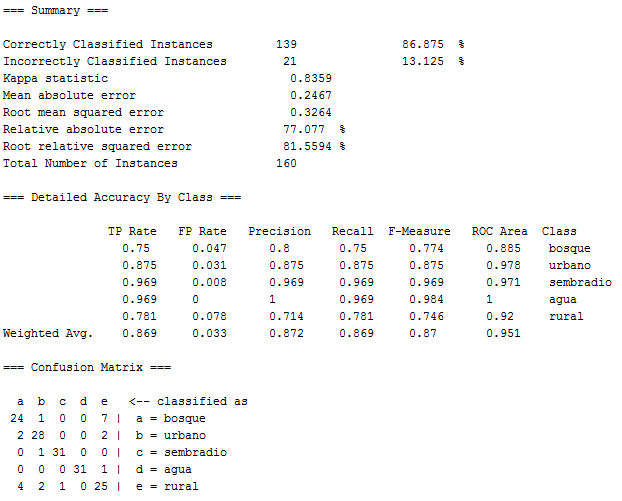
\includegraphics[width=1\textwidth]{images/salida-SMO.png}
    \caption{Fragmento de la salida de un clasificador SMO en Weka. Se pueden identificar datos importantes como el número y porcentaje de instancias clasificadas correcta e incorrectamente, la matriz de confusión y un bloque detallando la precisión por categoria.}
    \label{fig:salida-SMO}
\end{figure}

\subsection{Cálculo de Precisión}

La métrica de precisión que se utilizó para medir el desempeño de este experimento fue provista por el mismo Weka. El estadístico \textit{correctly classified instances} muestra tanto la cantidad de imágenes clasificadas correctamente así como un porcentaje. Este valor se calcula utilizando la matriz de confusión, como se muestra en la siguiente función:

\begin{equation}
  \text{Precisión} = \cfrac{ M_{1,1} + M_{2,2} + ... + M_{n,n}}{\text{Total de instancias}}
\end{equation}
Donde:
\begin{itemize}
    \item $M$ es la matriz de confusión.
    \item $n$ es el total de categorías, en este caso tipos de cobertura.
\end{itemize}
  

\subsection{Clasificadores}

Se seleccionaron cuatro clasificadores para evaluar la precisión. Cada uno tiene una naturaleza distinta: agrupamiento, basado en funciones, regresión y teoría Bayesiana. A continuación se describen cada uno de los clasificadores.


\subsubsection{K-Means}

El primer clasificador es un algoritmo básico de agrupamiento (o \textit{clustering} en inglés), llamado \textbf{K-Means}\cite{MacQueen1967}.

A grandes rasgos, este algoritmo interpreta cada arreglo de TF como un vector euclidiano en un espacio $n$-dimensional. Sobre este espacio se lanzan $k$ puntos, los \textit{centroides}, de manera aleatoria. 
Posteriormente, se hacen $i$ iteraciones en las cuales se miden los vectores más cercanos a cada centroide el cual se reposiciona hacia el centro de los vectores cercanos.
La idea es que luego de varias pasadas, los centroides irán gravitando hacia el centro de las nubes de puntos que representan las categorías (en este caso imágenes).

En Weka, la implementación de K-Means se denomina ``simpleKMeans''. Los parámetros de ejecución fueron:
\begin{itemize}
    \item Uso de todo el conjunto de datos para entrenamiento.
    \item 500 iteraciones.
    \item Uso de distancia euclidiana para el cálculo de cercanía.
\end{itemize}


\subsubsection{Máquina de Soporte Vectorial}

El segundo clasificador es un algoritmo de aprendizaje automático llamado \textbf{Máquina de Soporte Vectorial} (o \textit{Support Vector Machine} en inglés), en este caso particular usando el algoritmo de Optimización Secuencial Mínima\cite{Platt1999} (SMO por sus siglas en inglés).
Las Máquinas de Soporte Vectorial se utilizan normalmente en datos con alta dimensionalidad. Aquí, los datos se intentan dividir (clasificar) por medio de un hiperplano. Este plano no siempre existe por lo que los datos son transformados por una función no lineal llamada \textit{kernel} con el fin de facilitar su determinación.
En Weka, este algoritmo se denomina ``SMO'' y sus parámetros de ejecución fueron:
\begin{itemize}
    \item Entrenamiento usando Validación Cruzada de 10 iteraciones. Esta técnica se muestra en la figura \ref{fig:cross-validation}.
    \item Función \textit{Kernel} polinomial.
    \item Error aceptable de $1.0 \times 10^{-12}$.
    \item Normalización de los datos.
\end{itemize}

\begin{figure}
    \centering
    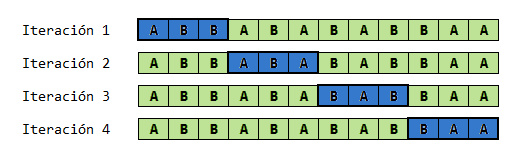
\includegraphics[width=0.75\textwidth]{images/cross-validation.png}
    \caption{Técnica de Validación Cruzada de 4 iteraciones. El conjunto de datos está compuesto por ítemes de los grupos A y B. En cada iteración, el grupo de elementos en azul se usa para validación y el grupo en verde para entrenamiento. Estos grupos van rotando tantas veces como iteraciones se dispongan.}
    \label{fig:cross-validation}
\end{figure}


\subsubsection{Regresión}

El siguiente clasificador sigue un modelo aditivo generalizado, (o \emph{boosting} en inglés). 
Esta técnica transforma un algoritmo débil en uno robusto al aplicarlo en sucesiones e ir ajustando una serie de pesos a lo largo de cada iteración. 
El algoritmo debil utilizado en este caso es la clásica técnica estadística de regresión, particularmente la regresión logística. La implementación de esta técnica se denomina \textbf{LogitBoost}\cite{Friedman2000}. En Weka se conoce con el mismo nombre y se utilizó con los parámetros por defecto.


\subsubsection{Redes bayesianas}

El último clasificador es el algoritmo de \textbf{red bayesiana}\cite{Bouckaert2008}. Las redes bayesianas son un modelo probabilístico que representa un conjunto de variables aleatorias y las condiciones de sus dependencias a través de un grafo dirigido cuyas aristas son probabilidades de que,  dada una variable, se dé otra. En el caso de la TT, se debe entender cada TF como una variable aleatoria y la red bayesiana intenta mapear las dependencias entre cada TF con el fin de maximizar la probabilidad de que todo el vector corresponda con la imagen original.
En Weka se denomina ``BayesNet'' y se usó con los parámetros por defecto.


